\documentclass[usenames,dvipsnames]{beamer}
\let\textmdorig\textmd
\let\textscorig\textsc
\let\textttorig\texttt

\mode<presentation> {
    \usetheme{metropolis}
%\setbeamertemplate{navigation symbols}{} % To remove the navigation symbols from the bottom of all slides uncomment this line
}
\usepackage[T1]{fontenc}
\usepackage{stmaryrd}
\usepackage{tikz}
\usepackage{tikz-3dplot}
\usetikzlibrary{calc}
\usepackage{dsfont}

\newcommand{\tikzmark}[1]{\tikz[overlay,remember picture] \node (#1) {};}

\usepackage[normalem]{ulem}
\usepackage{algpseudocode}
\usepackage{algorithm}
%\usepackage{algorithmic}
\usepackage{graphicx} % Allows including images
\usepackage{booktabs} % Allows the use of \toprule, \midrule and \bottomrule in tables

\usepackage{multirow}
\usepackage{xcolor}
\usepackage{colortbl}
\usepackage{xspace}
\usepackage{bbm}
\usepackage{amsfonts}
\usepackage{amsmath}
\usepackage{amssymb}
\usepackage{ulem}
\usepackage[backend=biber]{biblatex}
\bibliography{cites.bib}
\usefonttheme[onlymath]{serif}
%\usefonttheme{serif}
\setbeamertemplate{navigation symbols}{}

\newcolumntype{g}{>{\columncolor{black!5}}c}
\newcolumntype{f}{>{\columncolor{black!5}}r}
\newcolumntype{L}[1]{>{\columncolor{black!5}}m{#1}}
\usepackage{tikz}
\usetikzlibrary{shapes}
\usetikzlibrary{arrows}
\usetikzlibrary{positioning}
\usepackage[most]{tcolorbox}


\newenvironment{indentquote}{%
      \par%
        \medskip
          \leftskip=4em\rightskip=2em%
            \noindent\ignorespaces}{%
                  \par\medskip}

\newenvironment{indentquote2}{%
      \par%
        \medskip
          \leftskip=2em\rightskip=2em%
            \noindent\ignorespaces}{%
                  \par\medskip}


                  \title[CMR2Text]{AHH}

\author[Chris Kedzie]{Chris Kedzie and Kathleen McKeown} 
\institute[Columbia U.]
{
Columbia University\\
Department of Computer Science\\
\medskip
\textit{kedzie@cs.columbia.edu}
}
\date{\today} % Date, can be changed to a custom date


\makeatletter
\setbeamertemplate{title page}{
  \begin{minipage}[b][\paperheight]{\textwidth}
    \centering  % <-- Center here
    \ifx\inserttitlegraphic\@empty\else\usebeamertemplate*{title graphic}\fi
    \vfill%
    \ifx\inserttitle\@empty\else\usebeamertemplate*{title}\fi
    \ifx\insertsubtitle\@empty\else\usebeamertemplate*{subtitle}\fi
    \usebeamertemplate*{title separator}
    \ifx\beamer@shortauthor\@empty\else\usebeamertemplate*{author}\fi
    \ifx\insertdate\@empty\else\usebeamertemplate*{date}\fi
    \ifx\insertinstitute\@empty\else\usebeamertemplate*{institute}\fi
    \vfill
    \vspace*{1mm}
  \end{minipage}
}

\setbeamertemplate{title}{
%  \raggedright%  % <-- Comment here
  \linespread{1.0}%
  \inserttitle%
  \par%
  \vspace*{0.5em}
}
\setbeamertemplate{subtitle}{
%  \raggedright%  % <-- Comment here
  \insertsubtitle%
  \par%
  \vspace*{0.5em}
}
\makeatother

\newcommand\tocforsect[2]{%
      \begingroup
        \edef\safesection{\thesection}
          \setcounter{section}{#1}
            \tableofcontents[#2,currentsection]
              \setcounter{section}{\safesection}
                \endgroup
            }

\begin{document}

%\begin{frame}
%\titlepage 
%\end{frame}
\def\vc#1{$\vcenter{\hbox{#1}}$}
\begin{frame}
~\\
~\\
~\\
\resizebox{1.0\textwidth}{!}{%
{\begin{minipage}{0.90\textwidth}
{\Large
    $\textrm{Controllable}_\pi\left(\left[\!\!\!\left[ 
        \begin{array}{l} 
            \textrm{Meaning}\\\textrm{Representation}    
        \end{array} \right]\!\!\!\right]\right)$ }\\
   \vspace{0ex} $\quad \quad\quad \quad\quad \quad \quad\underrightarrow{\textrm{~~to~~}}$ 
         {\Large $\begin{array}{c} ~\\[-0.5em] \texttt{["Text", "Generation"]:} \end{array}$}\\
\end{minipage}}
}
~\\
\begin{center}---\\\textbf{Linearization and Data Augmentation Strategies}\\---\end{center}

    \usebeamertemplate*{title separator}
\begin{minipage}{0.5\textwidth}
\scriptsize
\uline{Chris Kedzie} and Kathleen McKeown\\
\scriptsize \textit{kedzie@cs.columbia.edu}
\end{minipage}\begin{minipage}{0.5\textwidth}
\raggedleft
\scriptsize Columbia University\\
\scriptsize Dept. of Computer Science
\end{minipage}
%\footnotesize Columbia University\\[-3pt]
%\footnotesize Department of Computer Science\\[7pt]
%\footnotesize \textit{kedzie@cs.columbia.edu}\\}

\end{frame}

\section{Background and Motivation}

\begin{frame}{Meaning Representation-to-Text Generation}
    \begin{center}
        \begin{tikzpicture}
            \node[anchor=north west] at (0,1.0)
                {\large \textbf{Input: Meaning Representation (MR)}};
            \only<1-6>{
                \node[anchor=north west] (mr) at (0,0) 
                    {$\left[\!\!\!\left[ \begin{array}{l} 
                        \textscorig{Inform} \\ 
                        \textrm{name=Aromi} \\ 
                        \textrm{eat\_type=coffee shop} \\ 
                        \textrm{area=city centre} \\ 
                    \end{array}\right]\!\!\!\right]$  };        
            }
            \only<7>{
                \node[anchor=north west] (mr) at (0,0) 
                    {$\left[\!\!\!\left[ \begin{array}{l} 
                        \textsc{Inform} \\ 
                        \textbf{\color{Red}name=Aromi} \\ 
                        \textbf{\color{Green}eat\_type=coffee shop} \\ 
                        \textbf{\color{Blue}area=city centre} \\ 
                    \end{array}\right]\!\!\!\right]$  };        
            }
            \only<2>{
                \draw[line width=0.75mm,->] (mr.south) -- (2.4,-3.5);

                \node[anchor=north west] (out) at (0,-4.0) 
                    {\large  \textbf{Output: Natural Language Utterance}};
                \node[anchor=north west,draw] (utt) at (0,-5.0) 
                    {\Large\textrm{For coffee in the city centre, try Aromi.}};
            }
            \uncover<7>{
                \draw[line width=0.75mm,->] (mr.south) -- (2.65,-3.5);

                \node[anchor=north west] (out) at (0,-4.0) 
                    {\large  \textbf{Output: Natural Language Utterance}};
                \node[anchor=north west,draw] (utt) at (0,-5.0) 
                {\Large\textrm{{\color{Green}\uline{\textbf{For coffee}}} 
                {\color{Blue}\uline{\textbf{in the city centre,}}} {\color{Red}\textbf{\uline{try Aromi.}}}}};
            }

    \uncover<3-5>{

        \node[anchor=north west,draw=mLightBrown,line width=0.5mm] (inform) at (0.43+0.05,-0.103) {\phantom{\textsc{Inform}}};
        \setbeamercolor{block title}{bg=mLightBrown,fg=white}
        \node[anchor=north west,text width=5cm,inner sep=0,outer sep=0] (da) at (5.0, -0.103) 
        {\vspace{-7.3pt}\begin{block}{Dialogue Act} 
                Goal/intent of the utterance
            \end{block}};
        \node[anchor=north west] (dafake) at (5.0,-0.103) {\phantom{\textsc{Inform}}};
        \draw[mLightBrown,thick] (inform.east) -- (dafake.west);
    }

            \uncover<4-5>{
                \node[anchor=north west,draw=Green,
                      line width=0.5mm,inner sep=0.8mm] (et) at (0.49,-1.248) 
                    {\phantom{\textrm{eat\_type}}};

                    \node[anchor=north west,line width=0.5mm,inner sep=0.8mm] 
                        (etfake1) at (-0.25,-1.248)  
                        {\phantom{\textrm{eat\_type}}};

                    \node[anchor=north west,line width=0.5mm,inner sep=0.8mm] 
                        (etfake2) at (-0.25,-3.25)  
                        {\phantom{\textrm{eat\_type}}};

                    \node[anchor=north west,line width=0.5mm,inner sep=0.8mm] 
                        (etfake3) at (0.25,-3.25)  
                        {\phantom{\textrm{eat\_type}}};

                \draw[Green,thick] (et.west) -- (etfake1.west) 
                    -- (etfake2.west) -- (etfake3.west);

                \setbeamercolor{block title}{bg=Green,fg=white}
        \node[anchor=north west,text width=4.2cm,inner sep=0,outer sep=0] (attr) at (0.0, -3.0) 
            {\begin{block}{Attributes} unordered, determines the semantics 
                of the MR\end{block}};
            }
            \uncover<5-5>{
                \node[anchor=north west,draw=VioletRed,line width=0.5mm]
                    (cc) at (1.50,-1.772) {\phantom{\textrm{city centre}}};
                \setbeamercolor{block title}{bg=VioletRed,fg=white}
                \node[anchor=north west,text width=4.0cm,inner sep=0,
                      outer sep=0] 
                    (val) at (5.0, -3.0) 
                    {\begin{block}{Attribute Values} 
                        \begin{itemize}
                            \item categorical \\ 
                            \item list-valued \\ 
                            \item free-text 
                        \end{itemize}\end{block}};

                \node[anchor=north west] (ccfake1) at (9.5, -1.772) 
                    {\phantom{\textrm{city centre}}};
                \node[anchor=north west] (ccfake2) at (9.5, -3.25) 
                    {\phantom{\textrm{city centre}}};
                \node[anchor=north west] (ccfake3) at (8.5, -3.25) 
                    {\phantom{\textrm{city centre}}};

                \draw[VioletRed,thick] (cc.east) -- (ccfake1.west) 
                    -- (ccfake2.west) -- (ccfake3.west);
            }
        \end{tikzpicture}
    \end{center}
\end{frame}

\begin{frame}{Controllable MR-to-Text Generation}
%            Surface realization order is determined by encoder, not the decoder language model.
%~\\
            
        \begin{center}
    \resizebox{0.95\textwidth}{!}{
    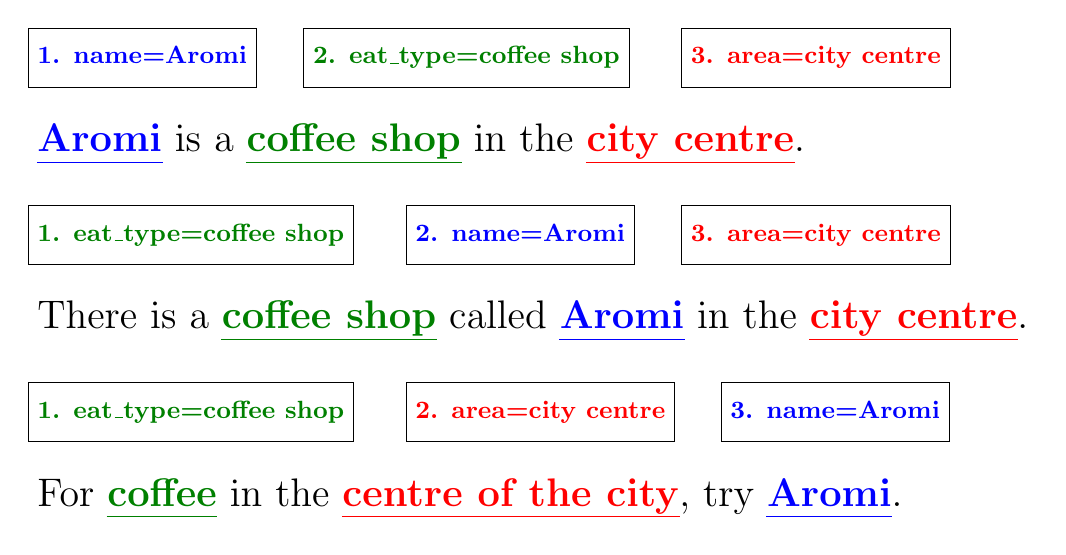
\begin{tikzpicture}
        \uncover<2->{
            \node[draw,anchor=north west,text=Blue,minimum height=0.75cm] at (0,0) {\small \textbf{1. name=Aromi\vphantom{p}}} ;
            \node[draw,anchor=north west,text=Green,minimum height=0.75cm] at (3.5,0) {\small \textbf{2. eat\_type=coffee shop}} ;
            \node[draw,anchor=north west,text=Red,minimum height=0.75cm] at (8.30,0) {\small \textbf{3. area=city centre}};
        \node[anchor=north west] at (0,-1.1) {\Large {\color{Blue}\uline{\textbf{Aromi}}} is a {\color{Green}\uline{\textbf{coffee shop}}} in the {\color{Red}\uline{\textbf{city centre}}}.};
    }
    \uncover<3->{
        \node[draw,anchor=north west,text=Green,minimum height=0.75cm] 
            at (0,-2.25) {\small \textbf{1. eat\_type=coffee shop}};
        \node[draw,anchor=north west,text=Blue,minimum height=0.75cm] 
        at (4.80,-2.25) {\small \textbf{2. name=Aromi\vphantom{p}}};
        \node[draw,anchor=north west,text=Red,minimum height=0.75cm] 
            at (8.3,-2.25) {\small \textbf{3. area=city centre}};
        \node[anchor=north west] at (0,-3.35) {\Large There is a {\color{Green}\uline{\textbf{coffee shop}}} called {\color{Blue}\uline{\textbf{Aromi}}} in the {\color{Red}\uline{\textbf{city centre}}}.} ;
    }
    \uncover<4->{
        \node[draw,anchor=north west,text=Green,minimum height=0.75cm] at (0,-4.5) {\small \textbf{1. eat\_type=coffee shop}};
        \node[draw,anchor=north west,text=Red,minimum height=0.75cm] at (4.8,-4.5) {\small \textbf{2. area=city centre}};
        \node[draw,anchor=north west,text=Blue,minimum height=0.75cm] at (8.8,-4.5) {\small \textbf{3. name=Aromi\vphantom{p}}} ;
        \node[anchor=north west] at (0,-5.6) {\Large For {\color{Green}\uline{\textbf{coffee}}} in the {\color{Red}\uline{\textbf{centre of the city}}}, try {\color{Blue}\uline{\textbf{Aromi}}}.} ;
    }



    \end{tikzpicture}
}
        \end{center}

\end{frame}





\begin{frame}{Controllable MR-to-Text Generation}


    Controllable MR-to-Text Generation will allow us to 
    \begin{itemize}
        \item implement more cognitively plausible
            discourse structuring models (e.g. Centering Theory or Accessibility Theory), 
\item more easily generate diverse outputs, and
\item confidently use neural components in NLG pipelines (Moryossef et al. (2019), Castro Ferreira et al. (2019))
    \end{itemize}
    


\end{frame}


\begin{frame}{Questions}
\begin{itemize}
\item Can you make an arbitrary sequence2sequence model controllable?
    \begin{itemize}
\item Are there differences between recurrent models or
transformers?
\item What about large pretrained models?
    \end{itemize} ~\\~\\
\item How systematic is a controllable sequence2sequence model? \\~\\
\item Can we improve systematicity with data-augmentation?~\\~\\
\end{itemize}
\end{frame}

\begin{frame}{Overview}
\tableofcontents[ 
    sectionstyle=show/show, 
    subsectionstyle=show/show, 
    ]
\end{frame}

\section{Controllable Generation}
\subsection{MR-to-Text with Seq2Seq}

\begin{frame}
\subsectionpage
\end{frame}

\begin{frame}{NLG as Seq2Seq}
   
    \resizebox{\textwidth}{!}{
    \begin{tikzpicture}
   \uncover<1-3>{
       \node[align=left,text width=10cm,anchor=north west] at (0,0) {\texttt{{\color{mLightBrown}\# Input}\\x = ?}};
   }

   \uncover<4>{
       \node[align=left,text width=10cm,anchor=north west] at (0,0) {\texttt{{\color{mLightBrown}\# Input}\\x = [\\~\\~\\~\\~\\~\\~\\]}};
   }
   \uncover<3-4>{
       \node[anchor=west] at (0.5,-2.8) 
       {\resizebox{5.5cm}{!}{$\uncover<4>{\pi\left(} \left[\!\!\!\left[ \begin{array}{l}
        \textsc{Inform}\\
        \textrm{name=Aromi}\\
        \textrm{eat\_type=coffee shop}\\
        \textrm{area=city centre}\\
    \end{array}\right]\!\!\!\right]\uncover<4>{\right)}$ }};


   }
   \uncover<4->{
       \node[text width=4.5cm,anchor=north west] at (0.5,-6) {A linearization strategy $\pi$ maps an MR to an equivalent sequence of tokens.};
   }
   \uncover<5->{
       \node[align=left,text width=10cm,anchor=north west] at (0,0) {\texttt{{\color{mLightBrown}\# Input}\\x = [\\
                    ~~~~"<<s>>",\\
                ~~~~"inform",\\
                ~~~~"name=Aromi",\\
                ~~~~"eat\_type=coffee shop",\\
                ~~~~"area=city centre",\\
                ~~~~"<<e>>"\\
            ]\\~
   }};
}
   \uncover<1>{
       \node[align=left,text width=5.75cm,anchor=north west] at (6.2,0) {\texttt{{\color{mLightBrown}\# Output}\\y = ?}};
   }
   \uncover<2->{
         \node[align=left,text width=5.75cm,anchor=north west] at (6.2,0) {\texttt{{\color{mLightBrown}\# Output}\\y = [\\ 
                    ~~~~"<start>",\\ 
                    ~~~~"for",\\
                    ~~~~"coffee",\\
                    ~~~~"in",\\
                    ~~~~"the",\\
                    ~~~~"city",\\
                    ~~~~"centre",\\ 
                    ~~~~",",\\
                    ~~~~"try",\\
                    ~~~~"aromi",\\
                    ~~~~".",\\
                    ~~~~"<stop>"\\
                ] \\ ~
   }};
   }

   \draw[mLightBrown!30] (6.2,0) -- (6.2,-8.15);
   \draw[mLightBrown!30] (0,0) -- (0,-4.85);
    \end{tikzpicture}
}
\end{frame}


\begin{frame}{NLG as Seq2Seq}

    \begin{center}
    \begin{tikzpicture}

        \node[draw=black,text width=3.5cm,minimum height=1.5cm,align=center] (enc) at (1.5,2) {Encoder};
        \node[draw=black,text width=3.5cm,minimum height=1.5cm,align=center] (dec) at (7.5,2) {Decoder};

        \draw[->] (enc.east) -- (dec.west);

        \node (x1) at (0,0) {$x_1$};
        \node (x2) at (1,0) {$x_2$};
        \node (x3) at (2,0) {$\cdots$};
        \node (xn) at (3,0) {$x_m$};


        \draw[->] (x1.north) -- +(0,1);
        \draw[->] (x2.north) -- +(0,1);
        \draw[->] (xn.north) -- +(0,1);

        \node (y1) at (6,0) {$y_1$};
        \node (y2) at (7,0) {$y_2$};
        \node (y3) at (8,0) {$\cdots$};
        \node (yn) at (9,0) {$y_{n-1}$};
        \draw[->] (y1.north) -- +(0,1);
        \draw[->] (y2.north) -- +(0,1);
        \draw[->] (yn.north) -- +(0,1);

        \node (o1) at (6,4) {$y_2$};
        \node (o2) at (7,4) {$y_3$};
        \node (o3) at (8,4) {$\cdots$};
        \node (on) at (9,4) {$y_{n}$};

        \draw[->] (o1)+(0,-1.25) -- (o1.south);
        \draw[->] (o2)+(0,-1.25) -- (o2.south);
        \draw[->] (on)+(0,-1.25) -- (on.south);

    \end{tikzpicture}
    \end{center}

Encoder/Decoder is either a GRU w/ Attention or Transformer.

\end{frame}



\subsection{Alignment Training}

\begin{frame}
    \alert{Alignment Training}

\end{frame}

\begin{frame}{Alignment Training}
   
    \resizebox{\textwidth}{!}{
    \begin{tikzpicture}

   \uncover<1-5>{
       \node[align=left,text width=10cm,anchor=north west] at (0,0) {\texttt{{\color{mLightBrown}\# Input}\\x = [\\~\\~\\~\\~\\~\\~\\]}};
   }
   \uncover<1-2>{
       \node[anchor=west] at (0.5,-2.8) 
       {\resizebox{5.5cm}{!}{$\pi = \left( \left[\!\!\!\left[ \begin{array}{l}
        \textsc{Inform}\\
        \textrm{\only<2>{\color{Red}}name=Aromi}\\
        \textrm{\only<2>{\color{Green}}eat\_type=coffee shop}\\
        \textrm{\only<2>{\color{Blue}}area=city centre}\\
    \end{array}\right]\!\!\!\right]\right)$ }};

   }
   \uncover<3>{
       \node[align=left,text width=10cm,anchor=north west] at (0,0) {\texttt{{\color{mLightBrown}\# Input}\\x = [\\
                    ~~~~"<start>",\\
                ~~~~"inform",\\
                ~~~~{\color{Green}"eat\_type=coffee shop",}\\
                ~~~~{\color{Blue}"area=city centre",}\\
                ~~~~{\color{Red}"name=Aromi",}\\
                ~~~~"<stop>"\\
            ]\\~
   }};
}
   \uncover<5>{
       \node[align=left,text width=10cm,anchor=north west] at (0,0) {\texttt{{\color{mLightBrown}\# Input}\\x = [\\
                    ~~~~"<start>",\\
                ~~~~"inform",\\
                ~~~~{\color{Green}"eat\_type=coffee shop",}\\
                ~~~~{\color{Red}"name=Aromi",}\\
                ~~~~{\color{Blue}"area=city centre",}\\
                ~~~~"<stop>"\\
            ]\\~
   }};
}
   \uncover<1-3>{
         \node[align=left,text width=5.75cm,anchor=north west] at (6.2,0) {\texttt{{\color{mLightBrown}\# Output}\\y = [\\ 
                    ~~~~"<start>",\\ 
                    ~~~~"for",\\
                    ~~~~\only<1>{"coffee",}\only<2->{{\color{Green}"coffee",}}\\
                    ~~~~"in",\\
                    ~~~~"the",\\
                ~~~~{\only<2->{\color{Blue}}"city",}\\
            ~~~~{\only<2->{\color{Blue}}"centre",}\\
                    ~~~~",",\\
                    ~~~~"try",\\
                ~~~~{\only<2->{\color{Red}}"aromi",}\\
                    ~~~~".",\\
                    ~~~~"<stop>"\\
                ] \\ ~
   }};
   }

   \uncover<4-5>{
         \node[align=left,text width=5.75cm,anchor=north west] at (6.2,0) {\texttt{{\color{mLightBrown}\# Output}\\y = [\\ 
                    ~~~~"<start>",\\ 
                    ~~~~"there",\\
                    ~~~~"is",\\
                    ~~~~"a",\\
                    ~~~~{{\color{Green}"coffee",}}\\
                    ~~~~{{\color{Green}"shop",}}\\
                    ~~~~"called",\\
                ~~~~{\color{Red}"aromi",}\\
                    ~~~~"in",\\
                    ~~~~"the",\\
                ~~~~{\color{Blue}"city",}\\
            ~~~~{\color{Blue}"centre",}\\
                    ~~~~".",\\
                    ~~~~"<stop>"\\
                ] \\ ~
   }};
   }


   \draw[mLightBrown!30] (6.2,0) -- (6.2,-8.15);
   \uncover<4-5>{
   \draw[mLightBrown!30] (6.2,0) -- (6.2,-9.21);
   }
   \draw[mLightBrown!30] (0,0) -- (0,-4.85);
    \end{tikzpicture}
}
\end{frame}



\subsection{Utterance Planning Models}

\begin{frame}
\subsectionpage
\end{frame}

\begin{frame}{What's the plan at test time?}

   
    \resizebox{\textwidth}{!}{
    \begin{tikzpicture}
   \draw[mLightBrown!30] (6.2,0) -- (6.2,-8.15);
   \draw[mLightBrown!30] (0,0) -- (0,-4.85);

   \uncover<1-2>{
       \node[align=left,text width=10cm,anchor=north west] at (0,0) {\texttt{{\color{mLightBrown}\# Input}\\x = [\\~\\~\\~\\~\\~\\~\\]}};
   }
   \uncover<1-2>{
       \node[anchor=west] at (0.5,-2.8) 
       {\resizebox{5.5cm}{!}{$\pi = \left( \left[\!\!\!\left[ \begin{array}{l}
        \textsc{Inform}\\
        \textrm{\color{Red}name=Aromi}\\
        \textrm{\color{Green}eat\_type=coffee shop}\\
        \textrm{\color{Blue}area=city centre}\\
    \end{array}\right]\!\!\!\right]\right)$ }};


   }
\uncover<1-2>{
    \draw[line width=1.5mm,draw=Green,<->] (5.4,-3.1) to [out=0,in=270] (6.15,-2.8) to [out=90,in=180] (6.8,-2.5);
\node at (4.25,-2.55) {};
    \draw[line width=1.5mm,draw=Red,<->] (4.20,-2.55) to [out=0,in=90] (6.15,-3.10) to [out=270,in=180] (6.70,-6.36);
    \draw[line width=1.5mm,draw=Blue,<->] (4.70,-3.56) to [out=0,in=180] (6.70,-4.36);
}
\uncover<2>{
    \node[color=Green,font=\Huge] at (7.1,-2.5) {\textbf{?}};
    \node[color=Red,font=\Huge] at (7.1,-6.36) {\textbf{?}};
    \node[color=Blue,font=\Huge] at (7.1,-4.36) {\textbf{?}};

   \node[font=\Huge,align=left,anchor=north west] at (8.0, -2) {\textbf{No reference} \\\textbf{utterance} \\\textbf{at test time!}};
}
         \node[align=left,text width=5.75cm,anchor=north west] at (6.2,0) {\texttt{{\color{mLightBrown}\# Output}\\y = [\\ 
                    \uncover<1>{~~~~"<<s>>",}\\ 
                    \uncover<1>{~~~~"for",}\\
                    \uncover<1>{~~~~{{\color{Green}"coffee",}}}\\
                    \uncover<1>{~~~~"in",}\\
                    \uncover<1>{~~~~"the",}\\
                    \uncover<1>{~~~~{\color{Blue}"city",}}\\
                    \uncover<1>{~~~~{\color{Blue}"centre",}}\\
                    \uncover<1>{~~~~",",}\\
                    \uncover<1>{~~~~"try",}\\
                    \uncover<1>{~~~~{\color{Red}"aromi",}}\\
                    \uncover<1>{~~~~".",}\\
                    \uncover<1>{~~~~"<<e>>"}\\
                ] \\ ~
   }};

    \end{tikzpicture}
}
\end{frame}

\begin{frame}{Utterance Planners}

\textbf{Bigram Utterance Planner} (\textsc{BgUP})\\
\begin{itemize}
\item Use training data to estimate bigram LM over attribute-value sequeunces.\\
~\\
$p(\textit{<<s>>})\times p(\textit{eat\_type=coffee shop}|\textit{<<s>>})\times p(\textit{area=city centre}|\textit{eat\_type=coffee shop})
\times p(\textit{name=Aromi}|\textit{area=city centre})\times
p(\textit{<<e>>}|\textit{name=Aromi})$\\~\\

\item Use constrained beam search to generate a candidate plan from an MR.
\end{itemize}
\end{frame}


\begin{frame}{Utterance Planners}

\textbf{Neural Utterance Planner} (\textsc{NUP})\\
Train a seq2seq model to map:
\begin{center}\vspace{-12pt}\small Arbitrary Linearization $\rightarrow$ Alignment Training\end{center}

\resizebox{\textwidth}{!}{
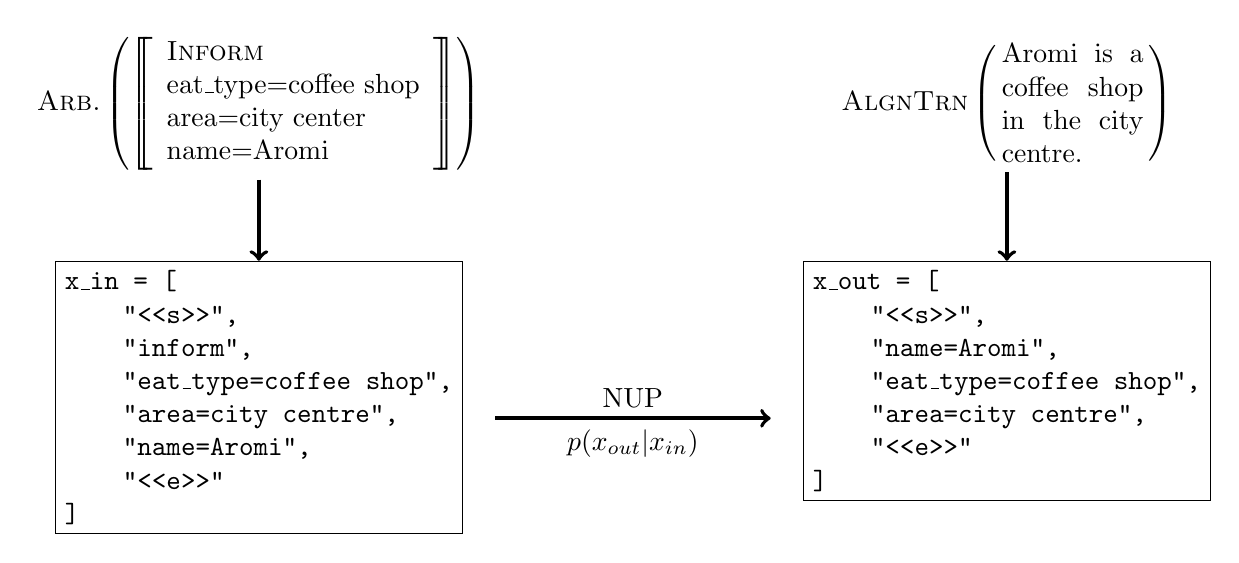
\begin{tikzpicture}
    \node (mr) at (0, 1) {$\textsc{Arb.}\left(\left[\!\!\!\left[
        \begin{array}{l}
            \textsc{Inform}\\
            \textrm{eat\_type=coffee shop}\\ 
            \textrm{area=city center} \\ 
            \textrm{name=Aromi}
        \end{array}\right]\!\!\!\right]\right)$};
    \node (utt) at (9.5,1) {$\textsc{AlgnTrn}\left(\, {\begin{minipage}{1.8cm}Aromi is a coffee shop in the city centre.\end{minipage}} \,\right)$ };
    \node[align=left,anchor=north,draw] (xin) at (0,-1) {
        \texttt{x\_in = [}\\
            \texttt{~~~~"<<s>>",}\\
            \texttt{~~~~"inform",}\\
            \texttt{~~~~"eat\_type=coffee shop",}\\ 
            \texttt{~~~~"area=city centre",} \\ 
            \texttt{~~~~"name=Aromi",} \\ 
            \texttt{~~~~"<<e>>"}\\
            \texttt{]}};


    \node[align=left,anchor=north,draw] (xout) at (9.5,-1) {
        \texttt{x\_out = [}\\
            \texttt{~~~~"<<s>>",}\\
            \texttt{~~~~"name=Aromi",} \\ 
            \texttt{~~~~"eat\_type=coffee shop",}\\ 
            \texttt{~~~~"area=city centre",} \\ 
            \texttt{~~~~"<<e>>"}\\
            \texttt{]}};

    %\texttt{["<<s>>",\\ "inform",\\ "eat\_type=coffee shop",\\ "area=city centre",\\ "name=Aromi", \\ "<<e>>"]}};

%    \node[align=center] (b) at (0,-4) {\texttt{["<<s>>", "name=Aromi", "eat\_type=coffee shop", "area=city centre", "<<e>>"]}};

%    \draw[line width=0.05cm,->] (a) to (b);
\draw [line width=0.05cm,->] (mr.south) to (xin.north);
\draw [line width=0.05cm,->] (utt.south) to (xout.north);
\draw [line width=0.05cm,->] (3,-3) -- (6.5,-3) node[midway,above] {NUP}
node[midway,below] {$p(x_{out}|x_{in})$};
\end{tikzpicture}
}
\end{frame}

\begin{frame}{Utterance Planners}
    \textbf{Oracle}
    \begin{itemize}
        \item Use Alignment Training ordering obtained from test-set reference utterances.
        \item Assumes clairvoyant knowledge of the test set.
    \end{itemize}

\end{frame}

\subsection{Phrase-Based Data Augmentation}
\begin{frame}
    \subsectionpage
\end{frame}
\begin{frame}

    Our Hope: seq2seq models should respond ``systematically'' to novel permutations or combinations of attribute-values. 

    \begin{itemize}

        \item Prior work has show limited systematicity in neural models (Lake and Baroni, 2018).
        \item Data-augmentation can help improve systematicity (Andreas, 2019).
    \end{itemize}

\end{frame}

\begin{frame}{Phrase-based Data Augmentation}

    \begin{enumerate}
        \item Parse Training Data\\~\\
        \item Create additional training examples from constitutent phrases.
    \end{enumerate}

\end{frame}


%\begin{frame}
%\resizebox{\textwidth}{!}{
%\begin{tikzpicture}[sibling distance=10em,level distance=1cm,
%  tn/.style = {shape=rectangle, rounded corners,
%    draw, align=center,
%    top color=white, bottom color=blue!20}]]
%  \node[] {S}
%    child { node[] (IT) {NP} } 
%    child[draw=white] { node[] {} }
%    child { node {\alert<7->{VP}}
%      child { node (IS) {\alert<7->{VBZ}}  }
%      child { node (NOT) {\alert<7->{RB}} }
%      child { node {\alert<6->{ADVP}} 
%        child { node (AVAILABLE) {\alert<6->{ADV}} }   
%        child { node {\alert<5->{S}} 
%            child { node (TO) {\alert<5->{TO}} }
%            child { node {\alert<4->{VP}} 
%                child { node (PLAY) {\alert<4->{VB}}  }
%                child { node {\alert<3->{PP}} 
%                    child { node (ON) {\alert<3->{IN}}  }
%                    child { node {\alert<2->{NP}} child { node (STEAM) {\alert<2->{NNP}}     }  }
%                }
%            }
%        }
%            }}; 
%%        child { node {S} child { node {VP} 
%%            child { node {TO} child {node {to}}  }  
%
%
% %               }  }   } };
%
%    \node [minimum height=1.0cm,below=7cm of IT] (it) {\Large It};
%    \draw[-] (IT) -- (it);
%
%    \node [minimum height=1.0cm,below=6cm of IS] (is) {\Large \alert<7->{is}};
%    \draw[-] (IS) -- (is);
%
%    \node [minimum height=1.0cm,below=6cm of NOT] (not) {\Large \alert<7->{not}};
%    \draw[-] (NOT) -- (not);
%
%    \node [minimum height=1.0cm,below=5cm of AVAILABLE] (available) {\Large \alert<6->{available}};
%    \draw[-] (AVAILABLE) -- (available);
%
%    \node [minimum height=1.0cm,below=4cm of TO] (to) {\Large \alert<5->{to}};
%    \draw[-] (TO) -- (to);
%
%    \node [minimum height=1.0cm,below=3cm of PLAY] (play) {\Large \alert<4->{play}};
%    \draw[-] (PLAY) -- (play);
%
%    \node [minimum height=1.0cm,below=2cm of ON] (on) {\Large \alert<3->{on}};
%    \draw[-] (ON) -- (on);
%
%    \node [minimum height=1.0cm,below=1cm of STEAM] (steam) {\Large \alert<2->{Linux}};
%    \draw[-] (STEAM) -- (steam);
%
%\uncover<2->{
%    \node[anchor=west] at (-3,-11) {\Large $\left[\!\!\!\left[ \begin{array}{l} \textsc{Inform}\\ \textrm{\alert<7>{has\_linux\_release=}\only<2-6>{yes}\only<7>{\alert{no}}}\end{array} \right]\!\!\!\right], \left[
%  \only<7>{\textit{<<s-VP>>}, \textit{is}, \textit{not}, \textit{available}, \textit{to}, \textit{play}, \textit{on},}
%  \only<6>{\textit{<<s-ADVP>>}, \textit{available}, \textit{to}, \textit{play}, \textit{on},}
%  \only<5>{\textit{<<s-S>>}, \textit{to}, \textit{play}, \textit{on},}
%  \only<4>{\textit{<<s-VP>>}, \textit{play}, \textit{on},} 
%    \only<3>{\textit{<<s-PP>>}, \textit{on},}    
%  \only<2>{\textit{<<s-NP>>},} \textit{linux}, \only<2>{\textit{<<e-NP>>}} 
%    \only<3>{\textit{<<e-PP>>}} 
%\only<4>{\textit{<<e-VP>>}} 
%\only<5>{\textit{<<e-S>>}} 
%\only<6>{\textit{<<e-ADVP>>}}
%\only<7>{\textit{<<e-VP>>}}
%\right]$};
%}
%
%\end{tikzpicture}}
\begin{frame}
\resizebox{\textwidth}{!}{
\begin{tikzpicture}[sibling distance=10em,level distance=1cm,
  tn/.style = {shape=rectangle, rounded corners,
    draw, align=center,
    top color=white, bottom color=blue!20}]]
  \node[] {S}
    child { node[] (IT) {NP} } 
    child[draw=white] { node[] {} }
    child { node {\alert<3->{VP}}
      child { node (IS) {\alert<3->{VBZ}}  }
      child { node (NOT) {\alert<3->{RB}} }
      child { node {\alert<2->{ADVP}} 
        child { node (AVAILABLE) {\alert<2->{ADV}} }   
        child { node {\alert<2->{S}} 
            child { node (TO) {\alert<2->{TO}} }
            child { node {\alert<2->{VP}} 
                child { node (PLAY) {\alert<2->{VB}}  }
                child { node {\alert<2->{PP}} 
                    child { node (ON) {\alert<2->{IN}}  }
                    child { node {\alert<2->{NP}} child { node (STEAM) {\alert<2->{NNP}}     }  }
                }
            }
        }
            }}; 
%        child { node {S} child { node {VP} 
%            child { node {TO} child {node {to}}  }  


 %               }  }   } };

    \node [minimum height=1.0cm,below=7cm of IT] (it) {\Large It};
    \draw[-] (IT) -- (it);

    \node [minimum height=1.0cm,below=6cm of IS] (is) {\Large \alert<3->{is}};
    \draw[-] (IS) -- (is);

    \node [minimum height=1.0cm,below=6cm of NOT] (not) {\Large \alert<3->{not}};
    \draw[-] (NOT) -- (not);

    \node [minimum height=1.0cm,below=5cm of AVAILABLE] (available) {\Large \alert<2->{available}};
    \draw[-] (AVAILABLE) -- (available);

    \node [minimum height=1.0cm,below=4cm of TO] (to) {\Large \alert<2->{to}};
    \draw[-] (TO) -- (to);

    \node [minimum height=1.0cm,below=3cm of PLAY] (play) {\Large \alert<2->{play}};
    \draw[-] (PLAY) -- (play);

    \node [minimum height=1.0cm,below=2cm of ON] (on) {\Large \alert<2->{on}};
    \draw[-] (ON) -- (on);

    \node [minimum height=1.0cm,below=1cm of STEAM] (steam) {\Large \alert<2->{Linux}};
    \draw[-] (STEAM) -- (steam);

\uncover<2->{
    \node[anchor=west] at (-3,-11) {\Large $\left[\!\!\!\left[ \begin{array}{l} \textsc{Inform}\\ \textrm{\alert<3>{has\_linux\_release=}\only<2-2>{yes}\only<3>{\alert{no}}}\end{array} \right]\!\!\!\right], \left[
                \only<3>{\textit{<<s-VP>>}, \alert{\textit{is}}, \alert{\textit{not}}, \textit{available}, \textit{to}, \textit{play}, \textit{on},}
  \only<2>{\textit{<<s-ADVP>>}, \textit{available}, \textit{to}, \textit{play}, \textit{on},}
  \textit{Linux},
\only<2>{\textit{<<e-ADVP>>}}
\only<3>{\textit{<<e-VP>>}}
\right]$};
}

\end{tikzpicture}}



\end{frame}

%
\newtcbox{\namebox}[1][]{enhanced, colframe=red, colback=red!15, 
                       nobeforeafter, tcbox raise base, shrink tight, extrude 
                       by=0.75mm, #1}
\newtcbox{\perspbox}[1][]{enhanced, colframe=blue, colback=blue!15, 
                       nobeforeafter, tcbox raise base, shrink tight, extrude 
                       by=0.75mm, #1}
\newtcbox{\rtsbox}[1][]{enhanced, colframe=green, colback=green!15, 
                       nobeforeafter, tcbox raise base, shrink tight, extrude 
                       by=0.75mm, #1}

\newtcbox{\psbox}[1][]{enhanced, colframe=orange, colback=orange!15, 
                       nobeforeafter, tcbox raise base, shrink tight, extrude 
                       by=0.75mm, #1}

\newtcbox{\pcbox}[1][]{enhanced, colframe=purple, colback=purple!15, 
                       nobeforeafter, tcbox raise base, shrink tight, extrude 
                       by=0.75mm, #1}

\newtcbox{\steambox}[1][]{enhanced, colframe=pink, colback=pink!15, 
                       nobeforeafter, tcbox raise base, shrink tight, extrude 
                       by=0.75mm, #1}

\newtcbox{\linuxbox}[1][]{enhanced, colframe=yellow, colback=yellow!15, 
                       nobeforeafter, tcbox raise base, shrink tight, extrude 
                       by=0.75mm, #1}

\newtcbox{\macbox}[1][]{enhanced, colframe=brown, colback=brown!15, 
                       nobeforeafter, tcbox raise base, shrink tight, extrude 
                       by=0.75mm, #1}

\section{Other Linearization Strategies}

\begin{frame}{Other Linearization Strategies}

\textit{\namebox{Age of Empires II} is a \perspbox{bird view}
\rtsbox{real-time strategy} game that
was released for \psbox{PlayStation}
and \pcbox{PC.} It \steambox{isn't available on Steam} 
and \linuxbox{doesn't have a Linux release}, 
but it \macbox{does have
a Mac version.}}

%\texttt{y = ["Age", "of", "Empires", "II", ":", "The", "Age", "of", "Kings", "is", "a", "bird", "view",
%"real-time", "strategy", "game", "that",
%"was", "released", "for", "PlayStation",
%"and", "PC", ".", "It", "is", "n't", "available", "on",
%"Steam", "and", "does", "n't", "have", "a",
%"Linux", "release", ",", "but", "it", "does", "have",
%"a", "Mac", "version", "."]}

\only<1>{
\texttt{x = [~~~~~~~~~~~~~~~~~~~~~~~~~~~~~\alert{\# \uline{Alignment Training}}\\
~~~~"inform",\\
~~~~"name=Age of Empires II",\\
~~~~"player\_perspective=bird view",\\
~~~~"genres=real-time strategy",\\
~~~~"platforms=PlayStation",\\
~~~~"platforms=PC",\\
~~~~"available\_on\_steam=no",\\
~~~~"has\_linux\_release=no",\\
~~~~"has\_mac\_release=yes"\\
]}
}

\only<2>{
\texttt{x = [~~~~~~~~~~~~~~~~~~~~~~\alert{\# \uline{Random}}\\
~~~~"inform",~~~~~~~~~~~~~~\alert{\# No correspondance between}\\
~~~~"platforms=PC",~~~~~~~~\alert{\# order of x and y. } \\
~~~~"player\_perspective=bird view",\\
~~~~"available\_on\_steam=no",\\
~~~~"genres=real-time strategy",\\
~~~~"name=Age of Empires II",\\
~~~~"has\_mac\_release=yes"\\
~~~~"platforms=PlayStation",\\
~~~~"has\_linux\_release=no",\\
]}
}

\only<3>{
\texttt{x = [~~~~~~~~~~~~~~~~~~~\alert{\# \uline{Increasing Frequency}}\\
~~~~"inform",~~~~~~~~~~~\alert{\# freq(x[i]) <= freq(x[i+1])}\\
~~~~"has\_linux\_release=no",\\
~~~~"has\_mac\_release=yes", \\
~~~~"available\_on\_steam=no",\\
~~~~"player\_perspective=bird view",\\
~~~~"platforms=PlayStation",\\
~~~~"platforms=PC", \\
~~~~"genres=real-time strategy",\\
~~~~"name=Age of Empires II",\\
]}
}
\only<4>{
\scalebox{0.5}{%
\begin{minipage}{0.7\textwidth}
\texttt{x = [\\
\phantom{oooo}"inform",\\
\phantom{oooo}"expected\_release\_data=N/A",\\
\phantom{oooo}"specifier=N/A",\\
\phantom{oooo}"has\_linux\_release=no",\\
\phantom{oooo}"has\_mac\_release=yes", \\
\phantom{oooo}"available\_on\_steam=no",\\
\phantom{oooo}"esrb\_rating=N/A",\\
\phantom{oooo}"has\_multiplayer=N/A",\\
\phantom{oooo}"developer=N/A",\\
\phantom{oooo}"release\_year=N/A",\\
\phantom{oooo}"player\_perspective1=bird view",\\
\phantom{oooo}"player\_perspective2=N/A",\\
\phantom{oooo}"player\_perspective3=N/A",\\
\phantom{oooo}"platforms1=PlayStation",\\
\phantom{oooo}"platforms2=PC", \\
\phantom{oooo}"platforms3=N/A", \\
\phantom{oooo}"platforms4=N/A", \\
\phantom{oooo}"name=Age of Empires II",\\
\phantom{oooo}"genres1=real-time strategy",\\
\phantom{oooo}"genres2=N/A",\\
\phantom{oooo}"genres3=N/A",\\
\phantom{oooo}"genres4=N/A",\\
]}
\end{minipage}}\begin{minipage}{0.5\textwidth} \texttt{\alert{\# Fixed Position}}\vfill ~\\~\\~\\ \end{minipage}} 
\end{frame}

\section{Experiments}
\begin{frame}{Experiments}
 \textbf{Models}   
\begin{itemize}
    \item biGRU w/ Attention
    \item Transformer
    \item BART (fine-tuned)
\end{itemize}

\textbf{Datasets}
\begin{itemize}
    \item E2E Challenge Dataset
    \item ViGGO Dataset
\end{itemize}
\end{frame}

\begin{frame}{Metrics}
some metrics
\end{frame}

\section{Conclusion}

\begin{frame}{Takeaways}
\begin{itemize}
\item Can you make an arbitrary sequence2sequence model controllable? 
    \\ \uncover<2->{\textbf{To some degree, Yes!}}

    \begin{itemize}
\item Are there differences between recurrent models or
    transformers? \\ \uncover<3->{\textbf{Recurrent models fair better in smaller data settings.}}
\item What about large pretrained models? \\ \uncover<4->{\textbf{These work great and you should use them when dataset is small.}}
    \end{itemize}
\end{itemize}
\end{frame}

\begin{frame}{Takeaways}
\begin{itemize}
\item How systematic is a controllable sequence2sequence model? \\
    \uncover<2->{\textbf{In the large data setting, pretty well!}}\\
    \uncover<3->{\textbf{In the small data setting, error increases on arbitrary plans.}}\\
    \uncover<4->{\textbf{The best bet is to fine-tune a large, pretrained LM.}}\\
\item Can we improve systematicity with data-augmentation?\\
    \uncover<5->{\textbf{Yes, but only really reliably on a large data setting, where we don't need to do it :( }}
\end{itemize}

\end{frame}

\begin{frame}{Thank You For Watching!}
add links to github and code/data/etc.
\end{frame}




\end{document}
